%%%%%%%%%%%%%%%%%%%%%%%%%%%%%%%%%%%%%%%%%%%%%%
%                insertmeeting
% 1) Title (something creative & funny?)
% 2) Date (MM/DD/YYYY)
% 3) Location (ex. Hagerty High School)
% 4) People/Committees Present 
% 5) Picture 
% 6) Start Time & Stop Time (ex. 12:30AM to 4:30PM)
%%%%%%%%%%%%%%%%%%%%%%%%%%%%%%%%%%%%%%%%%%%%%%
\insertmeeting 
	{Plenty of Planning (Again)} 
	{03/02/22} 
	{Hagerty High School}
	{James, Jensen, Nathan, Ritam}
	{Images/RobotPics/robot.jpg}
	{2:30 - 4:30}
	
\hhscommittee{General}
\noindent\hfil\rule{\textwidth}{.4pt}\hfil
\subsubsection*{Goals}
\begin{itemize}
    \item Plan for the rest of the week

\end{itemize} 

\noindent\hfil\rule{\textwidth}{.4pt}\hfil

\subsubsection*{Accomplishments}
Today our main goal was to plan for the rest of the week. This included writing packing lists, preparing team gifts, posters, and pit supplies for the competition. We also ensured each member turned in the required paperwork and forms for the trip. 


\begin{figure}[htp]
\centering
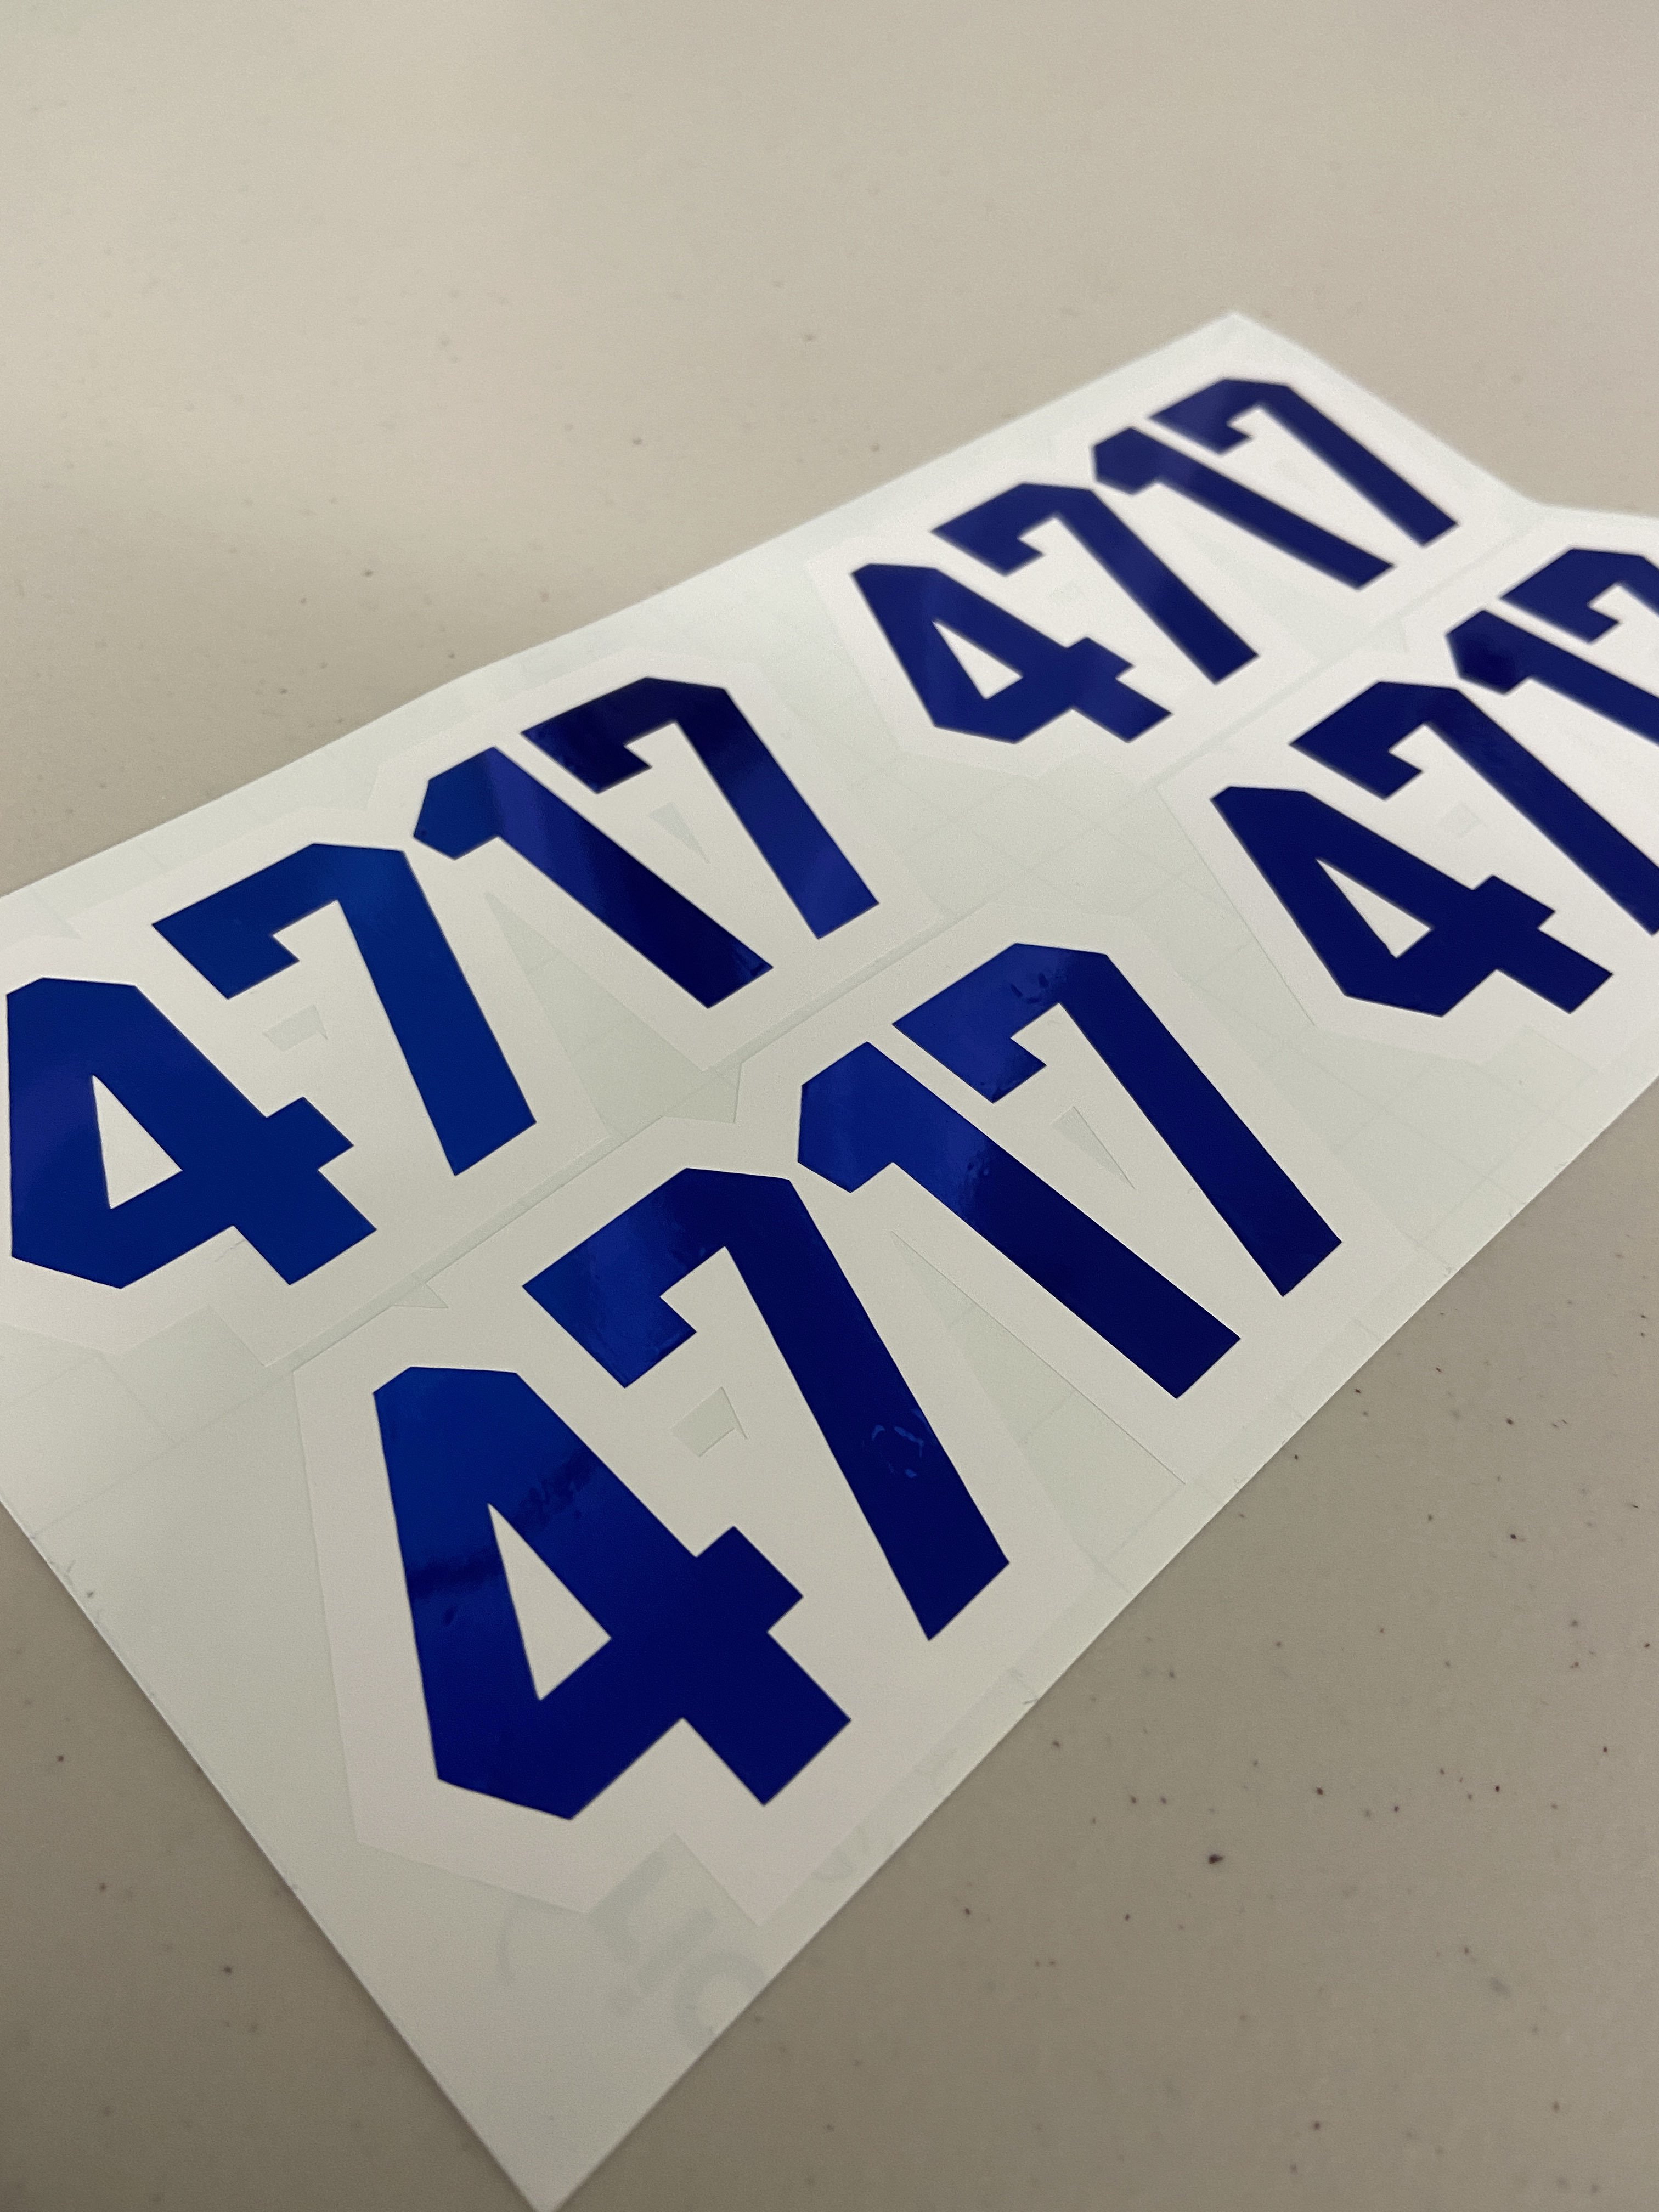
\includegraphics[width=0.95\textwidth, angle=0]{Meetings/March/03-01-22/03-01-22 1.jpg}
\caption{Our new robot team numbers}
\label{fig:030122_1}
\end{figure}

\begin{figure}[htp]
\centering
\includegraphics[width=0.95\textwidth, angle=0]{Meetings/March/03-01-22/03-01-22 2.jpg}
\caption{A set of lights to be used in pits}
\label{fig:030122_2}
\end{figure}

\begin{figure}[htp]
\centering
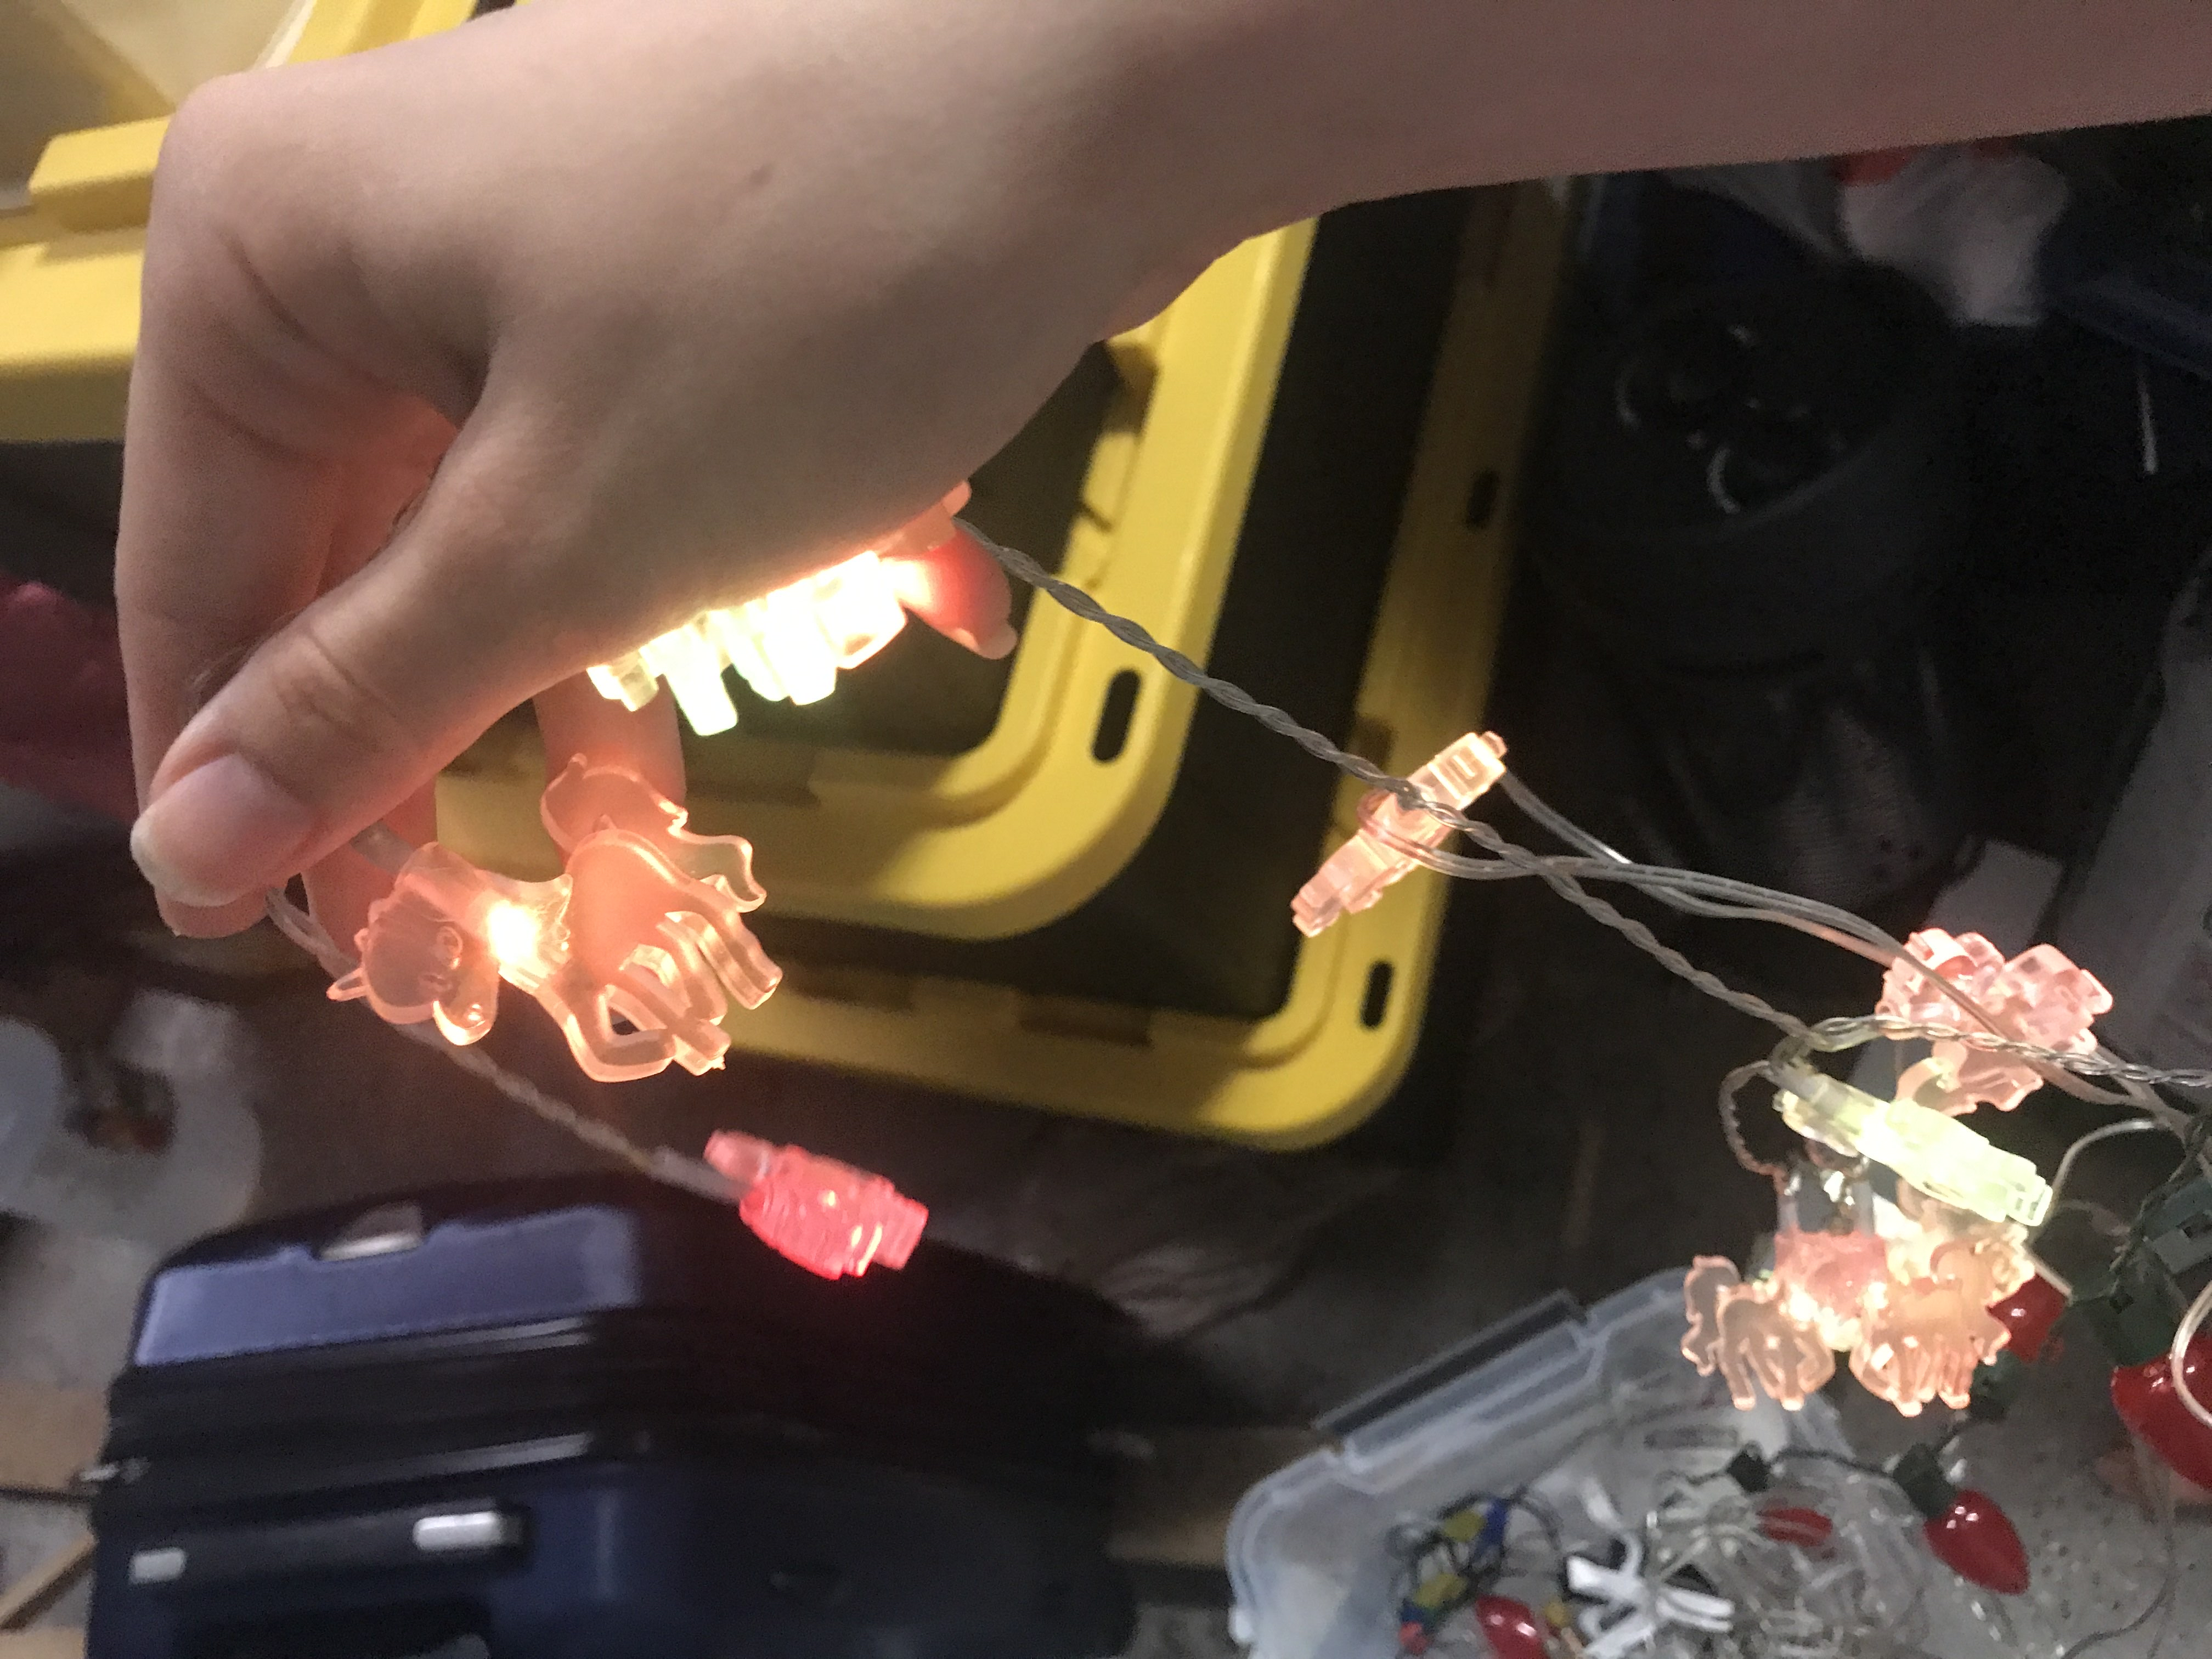
\includegraphics[width=0.95\textwidth, angle=0]{Meetings/March/03-01-22/03-01-22 3.jpg}
\caption{Unicorn lights for use in pits}
\label{fig:030122_3}
\end{figure}

\begin{figure}[htp]
\centering
\includegraphics[width=0.95\textwidth, angle=0]{Meetings/March/03-01-22/03-01-22 4.jpg}
\caption{Ducks with capes to give out at the competition}
\label{fig:030122_4}
\end{figure}


\whatsnext{
\begin{itemize}
    \item Prepare for this week's competition.
\end{itemize} 
}

